\level{2}{Applicazione Android}
    Il diagramma sottostante rappresenta la vista ad alto livello dell'applicazione Android.
   
    \begin{figure}[H]\centering
        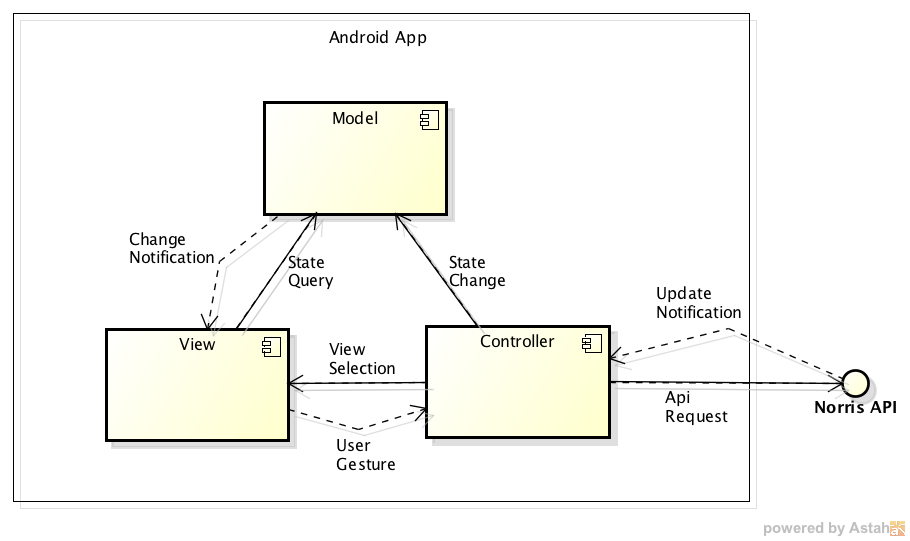
\includegraphics[width=\textwidth]{SpecificaTecnica/Pics/AndroidAppComponentDiagramLevel0.png}
        \caption{Diagramma delle componenti App Android}
    \end{figure}

    \level{3}{Descrizione delle componenti principali della app}
    	\level{4}{Model} 
        Il Model è il componente in cui sono contenute la struttura dei grafici e tutte le  informazioni inerenti ad essi, ovvero dati e impostazioni. In particolare contiene il modello di tutti i tipi di chart implementati nel framework. Questo componente permetterà solamente gli aggiornamenti consentiti dal modello chart utilizzato. Infine sarà possibile fare query sullo stato del modello.
       \level{4}{View}
        La View è il componente che rappresenta le varie UI dell'applicazione e i vari widget dei grafici da inserire nelle UI. In tale componente potrebbero esser sollevati degli eventi scatenati dall'utente.
       \level{4}{Controller}
        Questo componente ha il compito di gestire tutto il controllo dell'applicazione. Le operazioni che esso gestisce sono riassunte nel seguente elenco:
        	\begin{itemize}
        		\item crea il modello qualora questo sia necessario;
        		\item utilizza le API esterne di Norris;
        		\item interpreta i pacchetti ricevuti dal server contenenti i dati delle richieste API;
        		\item si mette in ascolto sul canale socket per ricevere gli aggiornamenti di stato dei chart;
        		\item interpreta i pacchetti di aggiornamento;
        		\item chiede al modello di aggiornare il suo stato;
        		\item richiede la creazione dei widget dei grafici da inserire nelle UI dell'applicazioe;
        		\item avvia le varie activity dell'applicazione;
        		\item gestisce le gesture dell'utente.
        \end{itemize}
    \level{2}{Descrizione delle interazioni che i componenti dell'app hanno tra di loro}
    	Le interazioni tra i componenti sono rappresentati con una freccia. Sono presenti due tipologie di frecce:
    	\begin{itemize}
    			\item{continua: } rappresenta l'invocazione di un metodo;
    			\item{tratteggiata: } rappresenta lo scatenarsi di un evento.
    		\end{itemize}
    	Le interazioni sono qui descritte:
    	\begin{description}
	    	\item{User Gesture:}
	    		La freccia etichettata con il termine "User Gesture" rappresenta l'evento scatenato dall'utente attraverso una gesture. Questo evento scatena nel controller la reazione lasciando ad esso il totale controllo su ciò che accade. Tale interazione si verifica per esempio quando l'utente seleziona un item della lista dei grafici presenti nell'istanza di Norris richiesta.
	    	\item{API Request:}
	    		L'applicazione Android dove interagire con il server dove è presente l'istanza Norris richiesta. Questa freccia rappresenta infatti le richieste delle API esterne di Norris da parte dell'applicazione (o più correttamente da parte del Controller) che ritorneranno un pacchetto con le informazioni richieste. Un esempio di tale richiesta è la richiesta dell'elenco dei grafici presenti nell'istanza di Norris. Per sapere quali sono le possibili API esterne fare riferimento al documento \insdoc{Analisi dei Requisiti v.X.xx}.
	    	\item{Update Notification:}
	    		Tale interazione rappresenta lo scatenarsi dell'evento di aggiornamento di un chart da parte del Server. Ogni aggiornamento infatti viene preso in carico dal Controller. Si verifica per esempio quando nel modello dati in Norris viene aggiunto un valore in un grafico.
	    	\item{State Change:}
	    		L'interazione etichettata con "State Change" rappresenta una richiesta, da parte del Controller al Model, di modifica dello stato. Tale modifica sarà la richiesta di aggiornamento dei dati nel modello.
	    	\item{Change Notification:}
	    		Questo evento viene scatenato dal modello quando il suo stato è stato modificato. Ha lo scopo di avvertire le varie View che osservano il modello che è avvenuta una modifica e devono quindi cambiare il loro stato.
	    	\item{State Query:}
	    		Questa interazione rappresenta la richiesta dello stato da parte della View verso il Model. Viene effettuata quando la View ha la necessità di esporre i dati del Model o qualcosa che sia dipendente dallo stato di quest'ultimo. Si ha una Query di questo genere per esempio quando il widget viene creato. Esso infatto dovrà recuperare i valori del chart per mostrarli.
	    	\item{View Selection:}
	    		Il controller ha il compito di scegliere quando e quale Activity visualizzare. Tale interazione rappresenta esattamente la richiesta di visualizzazione di una specifica Activity.
	    \end{description}

